
% Data acquisition comes prediction.  State-of-the-art data mining methods for software analytics include Synthetic Minority Oversampling Techniques (SMOTE) to handle class imbalance \cite{agrawal2018better, kamei12_jit} in combination with standard miners (Random Forest (RF), Logistic Regression (LR), and Support Vector Machine (SVM)). However, Chen et al. \cite{di18_fft} recommended Fast-Frugal Trees as the prediction model where it demonstrated that the model have dominated other standard methods for defect prediction and close issues prediction. Therefore, our recommended system to explore and improve the state-of-the-art risky software prediction of $F^3T$ as the combination of FASTREAD labeling method and FFTs predicting model will be validated with the comparisons against other standard data mining methods and answering the following research questions:

%         \textbf{RQ1: { How close are FASTREAD and Keyword Labeling to Human Labeling?}}
 
% Software maintenance is a continuing process, and software developers have the domain expertise in understanding the commit logs. 25,000+ commits are crossed labeled by SE Ph.D. students from 4 projects. With the initial assumption that software maintenance requires the expert's understanding, these human-labeled commit logs data from those four initial sampled repositories serves as the ground truth to compare the effectiveness of automatic Keywords versus FASTREAD tagging. FASTREAD statistically significant won across four cases with our three evaluation metrics of precision, recall, and false-alarms (up to 38\% precision, 31\% recall and 111\% false-alarm).
 
 %Four popular repositories that satisfy our sanity checks were picked at random, and their commit logs were sampled to be labeled for bug-fixing commits by a human. 

% \begin{RQ}{}
% \vspace{-10pt}

% FASTREAD as the method for bug-fixing commits augmentation is better than current automatic keyword tagging.
% \end{RQ}
 
 
%          \textbf{RQ2: { How are risky software commit prediction based on FASTREAD labeled data perform against state-of-the-art method (Keyword) labeled data?}}
  
% %From the bug-fixing commits, we can track back to find bug-inducing commits that introducing defects to the software. Each of these commits will be analyzed, and recommended metrics are extracted to describe how risky each commit is. 

% The right green flow in Figure \ref{fig:system} demonstrated our approach to improve the correctness of finding the bug-fixing commits. When the right bug-inducing commits are linked and analyzed to extract relevant values of metrics, a more robust model to predict future risky software commits is built. FFTs is validated as our chosen data miner when FFTs dominated the three standard methods (SMOTE+RF, SMOTE+LR, and SMOTE+SVM) in our experiment described in section 4 (RQ2). By winning 7 (78\%) for G-score and 6 (67\%) for $P_{\mathit{opt}}$ out of 9 projects, FFTs model built on FASTREAD labeled data outperform FFTs model built on Keyword labeled data. 
 

% \begin{RQ}{}
% \vspace{-10pt}
% FASTREAD labeled data are more fit and higher quality for risky software commit prediction. Automatic Keywords labeling method for defective software commit is deprecated for future defect prediction work.  
% \end{RQ}
  

%         \textbf{RQ3: {How state-of-the-art risky software commit identification and prediction system, Commit.Guru, comparing to our recommended $F^3T$ system in predicting risky software commit?}}
 
% %Data quality also comes from the proportion of the labels within the dataset. Agrawal et al. \cite{agrawal2018better} has found that imbalance class problem is apparent within defect prediction research. Although our study is not defect prediction, it does inherit a lot of defect prediction problem's nature where most of the commits are not bug-inducing commits. Risky software commit prediction also exhibit an imbalance class problem. Outside of data quality, data miner should be chosen carefully to leverage the nature of the problem and the dataset itself. 

% Current state-of-the-art risky software commit identification and prediction system is Commit.Guru (Keyword + Logistic Regression) that illustrated in the left blue flow in Figure \ref{fig:system}. However, FASTREAD is proven to improve the dependent features quality, or the correctness of risky software commit identification, the target for prediction task (from RQ1 and RQ2) while FFT has proven to be a robust data miner for software analytics task. Our proposed system of $F^3T$ (FASTREAD+FFTs) dominated on G-scores with statistically significants win on all 9 projects and improvement  of the absolute delta up to 48\%. For $P_{\mathit{opt}}$,  $F^3T$ won 7 out of 9 projects with the absolute delta up to 26\%. 

  
% \begin{RQ}{}
% \vspace{-10pt}
% $F^3T$ outperformed state-of-the-art risky software commit identification and prediction system, Commit.Guru. $F^3T$ is recommended as a new baseline for future research work.
% \end{RQ}

% %          extbf{RQ4: { How the FFT model comparing to state-of-the-art methods in predicting risky software commit?}}
 
% %  Modern state-of-the-art methods do include more than just Logistic Regression such as Random Forest (RF) and Support Vector Machine (SVM) for more complex problems in combination with Synthetic Minority Oversampling Technique (SMOTE) to handle class imbalance problem. It is essential to validate our data miner of choice FFT by comparing it against state-of-the-art data miners. With seven wins, one loss, and one tie, FFT model outperformed state of the art data miner in risky software commit prediction.  

 
% % \begin{RQ}{}
% % \vspace{-10pt}
% % FFT model outperformed state-of-the-art risky software commit prediction and is recommended as a new baseline for future work in risky software commit prediction.
% % \end{RQ}


% % \subsection{Experimental Rig}

% % \noindent         \textbf{Step 1: Bug-fixing commits augmentation.} For the initial four main projects (ABINIT, libMesh, MDANALYSIS, and LAMMPS), the commit logs are cross-labeled by two graduate students in SE research. Total of 9 projects are augmented by both automatic Keyword tagging method and FASTREAD method. 

% % \noindent         \textbf{Step 2: Bug-inducing change identification.} To link bug-fixing commits and their bug-inducing commits (e.g. crash, bug, issues), the well-known SZZ algorithm that is designed by Sliwerski and improved by Kim et al. is employed \cite{Sliwerski05changes, Kim08changes}.  

% % \noindent         \textbf{Step 3: Metrics Collection.} The recommended 14 metrics to study defect-prone commits by Kamei et al. \cite{kamei12_jit} from Table \ref{tbl:metrics} for each project are recorded by depriving from the source code control system (e.g., Git).  

% % \noindent         \textbf{Step 4: Data Preprocessing.} Current software analytics work include data transformation and prediction. Before experimenting with standard data miners, the data will be ``SMOTEd'' to handle class-imbalance, which was not considered in Commit.Guru. 

% % \noindent         \textbf{Step 5: Data Mining.} We adopted the incremental learning approach for this study where release $i$ of project $j$ is trained and test on release $i+1$. 
% % For the initial four projects (ABINIT, LIBMESH, LAMMPS, and MDANALYSIS), $j_i[keyword]$ and $j_i[FASTREAD]$ will be trained and test on $j_{i+1}[human]$. From that result, we are confident to scale up without human labels as ground-truth bug-fixing labels. 
% % Therefore, for the rest five projects, $j_i[keyword]$ and $j_i[FASTREAD]$ \hspace{0.05cm} will be trained to test on \hspace{0.05cm} $j_{i+1}[keyword]$ \hspace{0.05cm} and $j_{i+1}[FASTREAD]$ respectively. 
% % For this study, we comparing Fast-Frugal Trees against Support Vector Machine, Random Forest, and Logistic Regression (state-of-the-art data miner). The process is repeated 20 times to mitigate biases.  


% % \subsection{Systematic Commit Logs Labeling}

% % FASTREAD algorithm \cite{Yu2018} augmented bug-fixing commits by:
% % \begin{enumerate}
% %     \item Input thousands of commits per project.
% %     \item Initial random reasoning phase: humans to skim through the commits messages manually until they have found $|L_R| \geq 1$ bug-fixing commit (along with $|L_I|$ non bug-fixing ones). Dozens of both categories of commits should be found before next step.
% %     \item Reflective reasoning phase (Line 6-7 \cite{Yu2018})
% %     \bi
% %     \item The Support Vector Machine (SVM) model is trained on the $L$ examples. When $|L_R \leq 30|$, aggressive undersampling  are employed to reject all the non bug-fixing commits. 
% %     \item Uncertainty sampling of commits with highest uncertainty of category when $|L_R \leq 30|$ (line 25) and certainty sampling of commits with highest probability to be bug-fixing when $|L_R \geq 30|$ (line 27).   
% %     \item Iterate the reflective reasoning phase until more than 95\% of the bug-fixing commits have been found ($|L_R| \geq 0.95|R|$).
% %     \ei
% % \end{enumerate}




% %\subsection{Statistical Testing}

% %We compared our results of tuned miners per release version using statistical significance test and an effect size test by Scott-Knott procedure \cite{mittas2013ranking, ghotra15}. Significance test detects if two populations differ merely by random noises \cite{ghotra15}. Effect sizes checks whether two populations differ by more than just a trivial amount, where $\mathit{A12}$ effect size test was used \cite{arcuri2011practical}. Our stats test are statistically significant with 95\% confidence and not a ``small'' effect ($\mathit{A12} \ge 0.6$).



% \section{Results}



%         \textbf{RQ1: { How close are FASTREAD and Keyword Labeling to Human Labeling?}}
 
% Software maintenance is a continuing process and software developers have the domain expertise in understanding the commit logs. Four popular repositories (ABINIT, LAMMPS, LIBMESH, and MDANALYSIS) that satisfies our sanity checks were picked at random and their commit logs were sampled to be labeled for bug-fixing commits by human. With the initial assumption that software maintenance requires the expert's understanding, these human labeled commit logs data from those four repositories serves as the ground truth to compare the effectiveness of automatic keywords tagging versus FASTREAD tagging. Table \ref{tab:rq1} is very clear and we can conclude that FASTREAD won significantly on all three evaluations metrics (precision: 8\%-21\%, recall: 11\%-23\%, and especially in false-alarm 8\%-38\%). Interestingly, between false-alarm and recall relationship, if one metric is optimized, the other usually declined. However, from our initial results on just labeling comparing with manual human ground truths labels, FASTREAD labels to identify software bug-fixing commits are very close to how a developers would label them. 

% \begin{RQ}{}
% \vspace{-10pt}
% FASTREAD as the method for bug-fixing commits augmentation is better than current automatic keyword tagging.
% \end{RQ}





%         \textbf{RQ2: { How are risky software commit prediction based on FASTREAD labeled data perform against state-of-the-art method (Keyword) labeled data?}}
 


% % \begin{table}[!t]
% % \footnotesize
% % \begin{center}
% % \begin{tabular}{c@{~}|r@{~}|r@{~}|r@{~}|r@{~}}
% % \multicolumn{1}{c|}{} & \multicolumn{4}{c}{        \textbf{\% $P_{\mathit{opt}}$ Wins}} \\
% % \cline{2-5}
% % \begin{tabular}[c]{@{}c@{}}         \textbf{Dataset} \end{tabular} & \begin{tabular}[c]{@{}c@{}}            \textbf{SMOTE+RF}\end{tabular} &         \textbf{SMOTE+SVM} & \begin{tabular}[c]{@{}c@{}}         \textbf{SMOTE+LR}\end{tabular} &         \textbf{FFT} \\ \hline
% % PCMSOLVER & 0 & 0 & 0 & 0  \\ 

% % LAMMPS & 37 & 0 & 0 & 12  \\  

% % HOOMD & 0 & 0 & 0 & 20  \\  
% % MDANALYSIS & 28 & 0 & 0 & 28\\ 
% % XENON  & 16 & 0 & 0 & 33\\ 
% % ABINIT & 0 & 0 & 0 & 37 \\ 
% % LIBMESH & 12 & 0 & 0 & 50\\ 
% % AMBER & 0 & 33 & 0 & 66  \\ 
% % RMG-PY & 0 & 0 & 0 & 80\\ 

% % \end{tabular}
% % \end{center} 
% % \vspace{-10pt}
% % \end{table}

  
% From the bug-fixing commits, we can track back to find bug-inducing commits that introducing defects to the software. Each of these commits will be analyzed and recommended metrics are extracted to describe how risky each commit is. Finding the right bug-inducing commits will help to link to the right bug-inducing commits with appropriate values of metrics to build a strong model to predict future risky software commits. Our recommended data mining method is FFT with no preprocessing. Essentially, we wanted to compare $F^3T$ (FASTREAD+FFT) and Keyword+FFT.
 
 
 
%  In order to validate our chosen data miner, FFTs, we evaluated the performance of it by building FFTs on FASTREAD labeled data against standard methods (SMOTE+SVM, SMOTE+RF, and SMOTE+LR). Table \ref{tb:rq4} provides the statistical testing results for G-score (top) and $P_{\mathit{opt}}$ (bottom) performances. For G-score, FFT dominated in most of the releases, 7 wins out of 9 projects while performing similarly in 1 case (in AMBER) and losing to SMOTE+LR in 1 case (in PCMSOLVER) when 6 wins have 50\% and above win. For $P_{\mathit{opt}}$, FFT performance also have the most win percentages in most of the releases, 6 wins out of 9 projects while performing similarly to other data mining methods in 2 cases (PCMSOLVER and MDANALYSIS) and losing to SMOTE+RF in 1 case (in LAMMPS).  Figure \ref{fig:rq4} provides the median absolute delta performance insight from each project numerically between FFTs and state-of-the-art data mining methods (SMOTE+RF, SMOTE+SVM, and SMOTE+LR). We can see: (1) RF is widely adopted in defect prediction task but surprisingly doing worst in G-score (when comparing with FFTs for the median delta difference across all releases); (2) The good performance of SMOTE+LR when comparing to SMOTE+RF and SMOTE+SVM in G-score is evidental to why even though LR is deprecated in defect prediction task, it is widely adopted in JIT defect prediction \cite{commitguru}; (3) FFTs model outperformed standard data mining methods is validated as our chosen data miner. 


% % \begin{figure}[!t]
% % 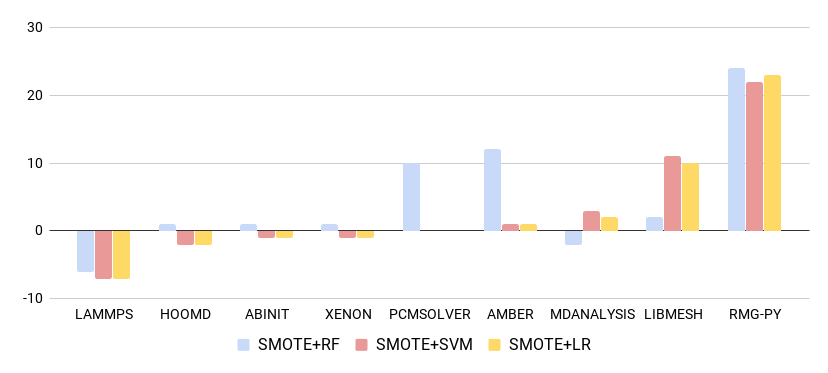
\includegraphics[width=\linewidth]{rq4_2.png}
% % \vspace{-25pt}
% % \end{figure}
 
% \begin{table}
% \small
% \begin{center}
% \caption{RQ2 Statistical Result - G-score (left) and $P_{\mathit{opt}}$ (right) percentage performance comparison of statistically significant wins across all the releases per project between FASTRERAD+FFT($F^3T$) versus Keyword+FFT(K+FFT)}
% \label{tb:rq2}
% \resizebox{\linewidth}{!}{
%  \begin{minipage}{0.55\linewidth}
% \begin{tabular}{c@{~}|r@{~}|r@{~}}
% \multicolumn{1}{c|}{} & \multicolumn{2}{c}{        \textbf{\% G-score Wins}} \\
% \cline{2-3}
% \begin{tabular}[c]{@{}c@{}}         \textbf{Dataset} \end{tabular} & \begin{tabular}[c]{@{}c@{}}         \textbf{K+FFT}\end{tabular} &         \textbf{$F^3T$}\\ \hline
% PCMSOLVER & 100 & 0  \\ 
% AMBER & 67 & 33  \\ 
% HOOMD & 40 & 60 \\ 
% RMG-PY  & 40 & 60 \\ 
%         \textbf{ABINIT} &         \textbf{25} &         \textbf{62} \\ 
%         \textbf{LIBMESH} &         \textbf{28} &         \textbf{72}  \\  
%         \textbf{MDANALYSIS} &         \textbf{28} &         \textbf{72} \\ 
%         \textbf{LAMMPS} &         \textbf{25} &         \textbf{75} \\
% XENON & 16 & 83  \\  
% \end{tabular}  %
% \end{minipage} \
% \begin{minipage}{0.55\linewidth}
% \begin{tabular}{c@{~}|r@{~}|r@{~}}
% \multicolumn{1}{c|}{} & \multicolumn{2}{c}{        \textbf{\% $P_{\mathit{opt}}$ Wins}} \\
% \cline{2-3}
% \begin{tabular}[c]{@{}c@{}} 
%         \textbf{Dataset} \end{tabular} & \begin{tabular}[c]{@{}c@{}}         \textbf{K+FFT}\end{tabular} &         \textbf{$F^3T$}\\ \hline
% AMBER & 67 & 33  \\
% HOOMD & 60 & 40 \\ 
% XENON & 50 & 50  \\  
%         \textbf{LAMMPS} &         \textbf{37} &         \textbf{50} \\
%         \textbf{ABINIT} &         \textbf{37} &         \textbf{50} \\ 
%         \textbf{MDANALYSIS} &         \textbf{42} &         \textbf{57} \\ 
% RMG-PY & 20 & 80 \\ 
%         \textbf{LIBMESH} &         \textbf{14} &         \textbf{86}  \\  
% PCMSOLVER & 0 & 100  \\ 
% \end{tabular}
% \end{minipage}}
% \end{center} 
% \vspace{-10pt}
% \end{table}




 
%  Figure \ref{fig:rq2} provides the median performance insight from each project for each release numerically between $F^3T$ and Keyword+FFT for G-score (top chart) and $P_{\mathit{opt}}$ (bottom chart). The blue diamond represents $F^3T$ while the black circle represents Keyword+FFT A lot of the differences between the two methods are easy to spot (i.e. performance on $P_{\mathit{opt}}$ chart for RMG-PY), but some are not (i.e. performance on G-score chart for AMBER). In order to confirm our hypothesis,
%  the percentage of statistically significant winning or ranking higher across all the releases in each project are recorded in Table \ref{tb:rq2}. Specifically, for LAMMPS, there are 9 releases, so the performance metrics are collected 8 times incrementally and FFT model built on FASTREAD generated data won 6/8 for G-score and 4/8 for $P_{\mathit{opt}}$  so $F^3T$ won 75\% time for G-score and 50\% for $P_{\mathit{opt}}$ in LAMMPS. The higher number between the twos is the better combination method. Four initial datasets that got human ground truth labels are expressed in bold entries. We observe that four out four, $F^3T$ statistically overwhelm Keyword+FFT using the "Human labeled" ground truths.  
 






% Manual human labeled ground truths are important for the data mining process but expensive to get and hard to repeat. Original four initial datasets provide plentiful evidence for us to have confidence in FASTREAD generated risky software prediction data. In order to confirm that hypothesis, the experiment is repeated without human ground truth labels by testing only on the next release that was generated from the same labeling method(i.e., a learner that was trained on ABINIT Keyword release 1 will predict on ABINIT Keyword release 2 and a learner that was trained on ABINIT FASTREAD release 1 will be tested on ABINIT FASTREAD release 2). It is similar to previous studies that solely using automating Keyword  \cite{nayrolles18_clever, commitguru}. 


% With 7 and 6 wins out of 9 projects for G-score and $P_{\mathit{opt}}$ respectively, FFTs model built on FASTREAD generated data outperformed FFTs model built on Keyword generated data. Hence, 

% \begin{RQ}{}
% \vspace{-10pt}
% FASTREAD labeled data are more fit and higher quality for risky software commit prediction. Automatic Keywords labeling method for defective software commit is deprecated for future defect prediction work.  
% \end{RQ}

% \begin{table}
% \small
% \begin{center}
% \caption{RQ3 Statistical Result - G-score (left) and $P_{\mathit{opt}}$ (right) percentage performance comparison of statistically significant wins across all the releases per project between $F^3T$ versus Commit.Guru}
% \label{tb:rq3}
% \resizebox{\linewidth}{!}{
%  \begin{minipage}{0.52\linewidth}
% \begin{tabular}{c@{~}|r@{~}|r@{~}}
% \multicolumn{1}{c|}{} & \multicolumn{2}{c}{        \textbf{\% G-score Wins}} \\
% \cline{2-3}
% \begin{tabular}[c]{@{}c@{}} \end{tabular} & 
% \begin{tabular}[c]{@{}c@{}}
%         \textbf{Commit}\end{tabular} & \\
%         \textbf{Dataset}  &          \textbf{Guru} &         \textbf{$F^3T$}\\\hline
% XENON & 16 & 66  \\ 
% LAMMPS & 0 & 75 \\ 
% HOOMD & 20 & 80 \\ 
% ABINIT  & 0 & 87 \\ 
% AMBER & 0 & 100 \\ 
% RMG-PY & 0 & 100 \\ 
% LIBMESH & 0 & 100 \\ 
% PCMSOLVER & 0 & 100 \\  
% MDANALYSIS & 0 & 100  \\ 
% \end{tabular} \qquad
% \end{minipage}
% \begin{minipage}{0.5\linewidth}
% \begin{tabular}{c@{~}|r@{~}|r@{~}}
% \multicolumn{1}{c|}{} & \multicolumn{2}{c}{        \textbf{\% $P_{\mathit{opt}}$ Wins}} \\
% \cline{2-3}
% \begin{tabular}[c]{@{}c@{}} \end{tabular} & \begin{tabular}[c]{@{}c@{}}         \textbf{Commit}\end{tabular} & \\
%         \textbf{Dataset}  &          \textbf{Guru} &         \textbf{$F^3T$}\\\hline
% PCMSOLVER & 100 & 0  \\ 
% AMBER & 67 & 33  \\ 
% HOOMD & 40 & 60 \\ 
% RMG-PY  & 40 & 60 \\ 
% ABINIT & 25 & 62 \\ 
% LIBMESH & 28 & 72  \\  
% MDANALYSIS & 28 & 72 \\ 
% LAMMPS & 25 & 75 \\
% XENON & 16 & 83  \\  

% \end{tabular}
% \end{minipage}}

% \end{center} 
% \vspace{-15pt}
% \end{table}

% % \begin{figure*}[!t]
% % \caption{RQ3 Numerical Results - Median G-score (top chart) and $P_{\mathit{opt}}$ (bottom chart) performance of comparing the performance between $F^3T$ and Commit.Guru for each release per project.}
% % 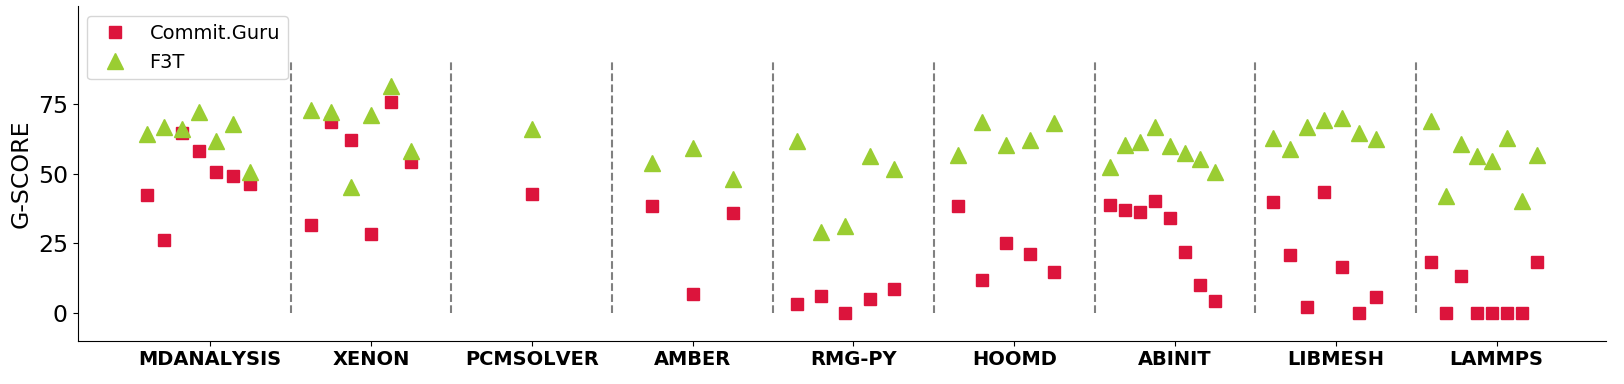
\includegraphics[width=\linewidth, height=1.8in]{rq3_1.png}
% % \label{fig:rq3}
% % \vspace{-20pt}
% % \end{figure*}
% % \begin{figure*}[!t]
% % 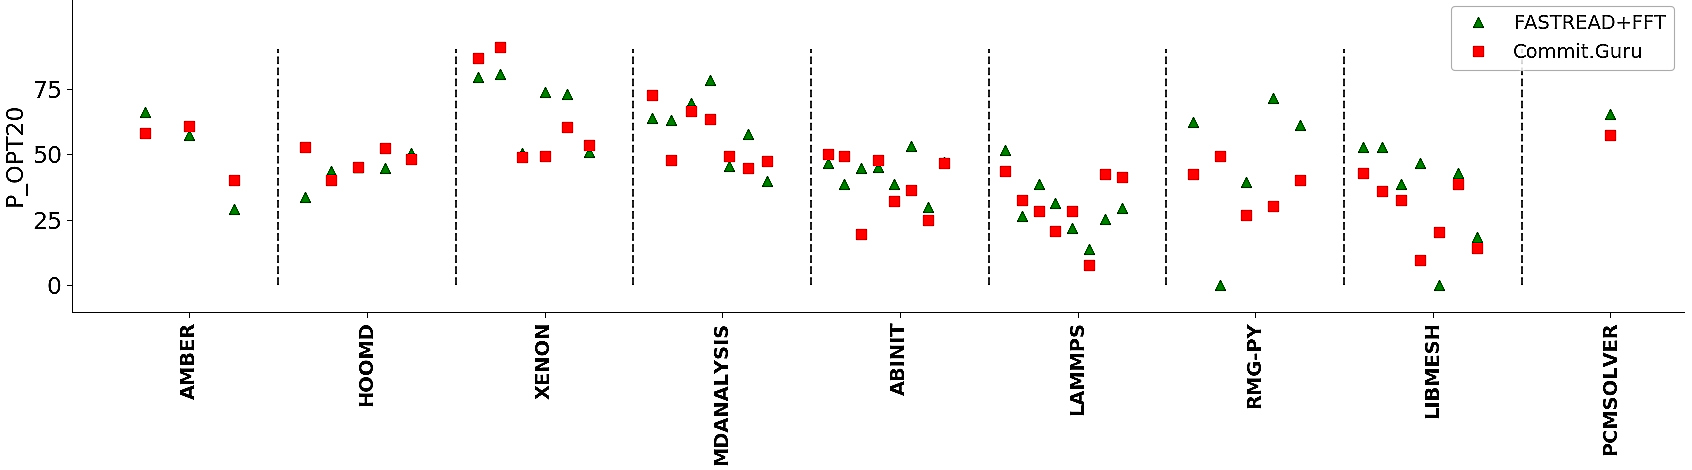
\includegraphics[width=\linewidth, height=1.8in]{rq3_2.png}
% % \vspace{-20pt}
% % \end{figure*}

% \textbf{RQ3: {How state-of-the-art risky software commit identification and prediction system, Commit.Guru, comparing to our recommended $F^3T$ system in predicting risky software commit?}}
 
% Beside dependent ground truth labels, data quality also comes from the proportion of the labels within the dataset. Agrawal et al. \cite{agrawal2018better} has found that the imbalance class problem is apparent within defect prediction research. Although, our study is not defect prediction, it does inherit a lot of defect prediction problem's nature where most of the commits are not bug-inducing commits as shown in Table \ref{tbl:dataset} where the median of defective commit is 23\%. Therefore, risky software commit also exhibit imbalance class problem. Outside of data quality, data miner should be chosen carefully to leverage the nature of the problem and the dataset itself. FASTREAD improves the dependent features quality or the correctness of risky software commit identification, target for prediction task (from RQ1 and RQ2) while FFTs model has proven to be a strong data miner for software analytics task. Our recommended $F^3T$ method is chosen for this paper to compare against state-of-the-art risky software prediction method, Commit.Guru's Keyword+LR. 

% From the Figure \ref{fig:rq3}, the green triangles and red squares represent $F^3T$'s performance and Commit.Guru's performance for G-score (top chart) and $P_{\mathit{opt}}$ (bottom chart). $F^3T$ clearly outperformed Keyword+LR on all 9 projects for G-score where $F^3T$ won 100\% of the time in 5 projects for all the releases within that same project (recorded Table \ref{tb:rq3}). For $P_{\mathit{opt}}$, $F^3T$ won 7 out of 9 projects with statistically significant differences in the right of Table \ref{tb:rq3}. With the majority won on both measures, we can conclude: 


% \begin{RQ}{}
% \vspace{-10pt}
% $F^3T$ outperformed state-of-the-art risky software commit identification and prediction system, Commit.Guru. $F^3T$ is recommended as a new baseline for future research work.
% \end{RQ}




% %         extbf{RQ4: { How FFT model comparing to state-of-the-art data mining methods in predicting risky software commit?}}
 
% % Modern state-of-the-art methods does include more than just Logistic Regression such as Random Forest and Support Vector Machine for more complex problems in the combination with Synthetic Minority Oversampling Technique (SMOTE) to handle class imbalance problem. It is essential to validate our data miner of choice (i.e. FFTs), by comparing against state-of-the-art data mining methods in SE research. 

% % \begin{figure}[!t]
% % \vspace{-10pt}
% % \caption{RQ4 Numerical Difference Result - Absolute median delta of G-score (top chart) and $P_{\mathit{opt}}$ (bottom  chart) of comparing the performances between FFTs and state-of-the-art methods (SMOTE+SVM, SMOTE+RF, and SMOTE+LR)}
% % 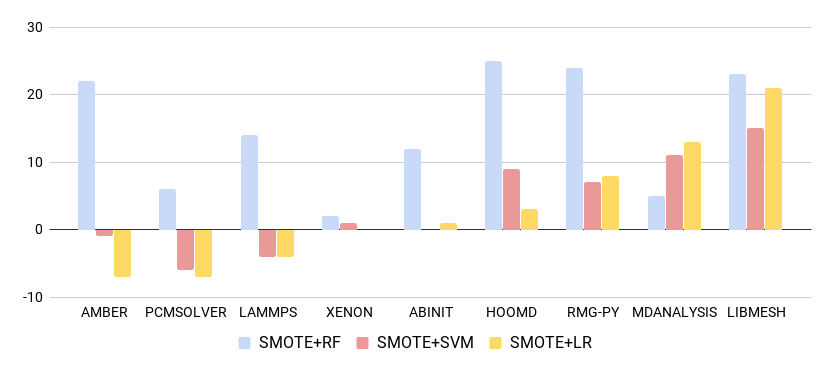
\includegraphics[width=\linewidth, height=1.8in]{rq4_1.png}
% % \label{fig:rq4}
% % \vspace{-25pt}
% % \end{figure}
% % \begin{figure}[!t]
% % 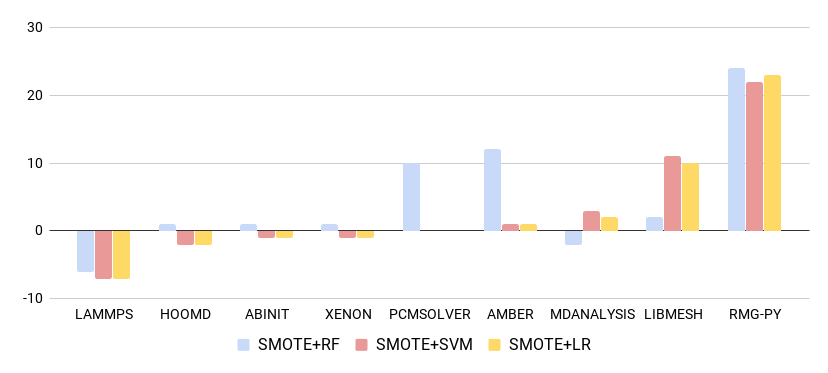
\includegraphics[width=\linewidth, height=1.8in]{rq4_2.png}
% % \vspace{-25pt}
% % \end{figure}

% % The experiment and evaluation are similar to RQ2 and RQ3 but only training and testing on FASTREAD generated data. Table \ref{tb:rq4} provides the statistical testing results for G-score (top) and $P_{\mathit{opt}}$ (bottom) performances of comparing FFTs with SMOTE+RF, SMOTE+SVM, and SMOTE+LR. For G-score, FFT dominated in most of the releases, 7 wins out of 9 projects while performing similarly in 1 case (in AMBER) and losing to SMOTE+LR in 1 case (in PCMSOLVER) when 6 wins have 50\% and above win. For $P_{\mathit{opt}}$, FFT performance also have the most win percentages in most of the releases, 6 wins out of 9 projects while performing similarly to other data mining methods in 2 cases (PCMSOLVER and MDANALYSIS) and losing to SMOTE+RF in 1 case (in LAMMPS).  Figure \ref{fig:rq4} provides the median absolute delta performance insight from each project numerically between FFTs and state-of-the-art data mining methods (SMOTE+RF, SMOTE+SVM, and SMOTE+LR). We can see: (1) RF is widely adopted in defect prediction task but surprisingly doing worst in G-score (when comparing with FFTs for the median delta difference across all releases); (2) The good performance of SMOTE+LR when comparing to SMOTE+RF and SMOTE+SVM in G-score is evidental to why even though LR is deprecated in defect prediction task, it is  widely adopted in JIT defect prediction \cite{commitguru}. Finally, 


% % \begin{RQ}{}
% % \vspace{-10pt}
% % FFT model outperformed state-of-the-art risky software commit prediction and is recommended as a new baseline for future work in risky software commit prediction.
% % \end{RQ}
